\documentclass[11pt]{article}
\usepackage[margin=1in]{geometry}
\usepackage[T1]{fontenc}
\usepackage{lmodern,amsmath,amssymb,booktabs,graphicx,microtype,xurl}
\usepackage[hidelinks]{hyperref}
\setlength{\emergencystretch}{3em}
\title{Coordination-Adjusted Architecture Selection\\for LLM Agent Systems:\\A Reproducible Decision Model and Simulation Benchmark}
\author{Goutham Siripuram\\Independent Researcher}
\date{October 12, 2026\\\small Methodology preprint; software version 0.3.0}
\begin{document}
\maketitle
\begin{abstract}
Choosing an LLM agent architecture requires assumptions about the value of decomposition, specialization, and verification relative to coordination, error propagation, and resource costs. This paper proposes an executable linear decision model over six normalized task descriptors and four architecture classes. All coefficients are hand-specified design hypotheses. A seeded generator supplies 48 synthetic scenarios with independently sampled features, and a sensitivity analysis reports how the resulting recommendations change with resource aversion. These calculations describe the behavior of the specified model; they do not measure agent performance or establish which architecture is best in practice. We make the coefficient table, tie policy, reproduction procedure, and identification limitations explicit, and outline training, held-out evaluation, and baseline comparisons needed for empirical calibration. The contribution is a transparent decision-model template and simulation artifact, not an empirically validated architecture selector.
\end{abstract}

\section{Introduction}
An agent architecture specifies how reasoning, tools, delegation, and checking are organized. ReAct illustrates reasoning interleaved with actions \cite{yao2023react}; Toolformer studies learned tool use \cite{schick2023toolformer}. These mechanisms do not determine how many coordinated roles a task needs. This paper provides a small decision-model template that makes proposed benefits and costs of architecture choices explicit.

The artifact evaluates four classes using six normalized descriptors and a hand-specified coefficient table. Its contribution is transparency and reproducible sensitivity analysis. It does not offer a trained selector, an empirical performance benchmark, or a claim that additional agents improve outcomes. The term simulation benchmark denotes fixed inputs for exercising the decision rule, without ground-truth best-architecture labels.

\section{Related work and scope}
Guo et al. survey LLM-based multi-agent systems and their organizational challenges \cite{guo2024multiagent}. Cemri et al. analyze failures involving system design, inter-agent misalignment, and task verification \cite{cemri2025failures}. These motivate explicit attention to coordination and error propagation, but do not supply numerical values for this model.

Kim et al. investigate architecture-task alignment and coordination through empirical scaling experiments \cite{kim2026scaling}. That work directly limits any novelty claim that architecture selection should consider overhead. The present contribution is a deliberately small, hand-specified linear template and executable simulation artifact. It has neither the empirical calibration nor the predictive evidence of an experimentally fitted model. We do not claim a new scaling law.

AgentBench \cite{liu2024agentbench}, WebArena \cite{zhou2024webarena}, WorkArena \cite{drouin2024workarena}, and OSWorld \cite{xie2024osworld} offer candidate environments for future controlled comparisons. No results from those benchmarks are reported here, and their existence does not validate our architecture labels, features, or coefficients.

\section{Problem formulation}
Let $\mathcal A$ contain a single agent (SA), a single agent with tools (SAT), a planner--executor--verifier (PEV), and a hierarchical multi-agent arrangement (HMA). These are conceptual labels in this artifact, not executable implementations. An empirical study would need to freeze concrete orchestration, communication, model, and tool configurations; the labels alone do not guarantee comparable capabilities.

The input vector is $x=(D,S,V,H,P,K)\in[0,1]^6$: decomposability, specialization need, verification value, coordination burden, error-propagation risk, and resource sensitivity. These are elicited descriptors, not directly measured probabilities. A possible future rubric could score decomposability by the fraction of independently checkable subtasks and coordination burden by dependency density, but no validated mapping of observations to these scales is provided here. Coordination and propagation also depend on architecture; using common task-level proxies and architecture-specific coefficients is a simplifying assumption.

\section{Decision model}
For architecture $a$ and nonnegative resource-aversion parameter $\lambda$, define
\begin{equation}\label{eq:utility}
U_a(x;\lambda)=\alpha_aD+\beta_aS+\gamma_aV-\delta_aH-\eta_aP-\lambda\zeta_aK.
\end{equation}
The proposed recommendation maximizes $U_a$. Table~\ref{tab:coefficients} gives all reference coefficients. They express a hypothetical preference structure; they were not fitted to observations. Utility may be negative and is neither a success probability nor a monetary estimate. The default is $\lambda=1$.

\begin{table}[htbp]\centering
\caption{Hand-specified coefficients. Values are design hypotheses, not estimated effects.}\label{tab:coefficients}
\begin{tabular}{lrrrrrr}
\toprule
Architecture & $\alpha$ & $\beta$ & $\gamma$ & $\delta$ & $\eta$ & $\zeta$ \\
\midrule
SA & 0.05 & 0.05 & 0.02 & 0.05 & 0.06 & 0.05 \\
SAT & 0.10 & 0.30 & 0.08 & 0.08 & 0.08 & 0.12 \\
PEV & 0.45 & 0.35 & 0.70 & 0.35 & 0.25 & 0.35 \\
HMA & 0.85 & 0.80 & 0.65 & 0.75 & 0.55 & 0.70 \\
\bottomrule
\end{tabular}

\end{table}

The implementation rejects nonfinite or out-of-range features, missing features, and nonfinite or negative $\lambda$. It computes all four utilities and finds every architecture within a nonnegative finite tolerance $\tau$ of the maximum, default $10^{-12}$. If more than one is within tolerance, it raises an explicit tie error. This prevents dictionary order from acting as an undocumented tie policy. An applied system would need a declared tie procedure, such as collecting more information or comparing a separately measured cost; no such procedure is inferred here.

\subsection{Interpretation and identification}
For two architectures, the utility difference is linear in the descriptors, so boundaries of indifference are hyperplanes. Holding the other features fixed gives $\partial U_a/\partial\lambda=-\zeta_aK$. Thus increasing $\lambda$ cannot increase any architecture's utility for $K\geq0$, though it can change which architecture wins. This is a consequence of the equation, not a finding about real agent costs.

Weights and feature scales are jointly underidentified without measurement conventions. Multiplying all coefficients by a common positive number preserves exact argmax rankings, though numerical tolerance must scale accordingly. Different rubrics or interaction terms can change rankings. Reporting only the recommended label hides small margins; the reproduction script therefore saves all utilities as well as selections.

\section{Synthetic scenario design}
The version 0.2 generator supplies 48 scenarios. Python's \texttt{random.Random(260907)} draws each of the six coordinates separately from a uniform distribution and rounds it to six decimal places. The released rows carry a synthetic flag. This removes the earlier deterministic coupling of favorable decomposition with low coordination burden. Independent generation does not imply zero sample correlation in a finite file, nor does it show that real task descriptors are independent.

There are no measured task outcomes, LLM calls, or best-architecture labels. Scenario count is a convenience for exercising the code, not a power calculation. The generator and all feature values are included in the repository. Sensitivity analysis evaluates the same scenarios at $\lambda\in\{0,0.5,1,2,4\}$ while retaining every other input and coefficient.

\section{Illustrative simulation results}
Table~\ref{tab:recommendations} reports recommendation counts. Each column total is 48. These frequencies describe how the reference coefficients partition this synthetic input set. A frequent recommendation is not evidence that its architecture performs better or is more prevalent in a real workload.

\begin{table}[htbp]\centering
\caption{Synthetic selection counts under different resource-aversion settings. No empirical architecture-performance comparison.}\label{tab:recommendations}
\begin{tabular}{lrrrrr}
\toprule
Architecture & $\lambda=0$ & $0.5$ & $1$ & $2$ & $4$ \\
\midrule
SA & 0 & 0 & 1 & 1 & 13 \\
SAT & 3 & 5 & 4 & 11 & 10 \\
PEV & 12 & 16 & 21 & 22 & 20 \\
HMA & 33 & 27 & 22 & 14 & 5 \\
\bottomrule
\end{tabular}

\end{table}

Figure~\ref{fig:sensitivity} displays the same calculation. Changes are expected because the four resource coefficients differ. The artifact does not estimate an optimal $\lambda$; such a choice would require an externally justified tradeoff between measured quality and resources.
\begin{figure}[htbp]\centering
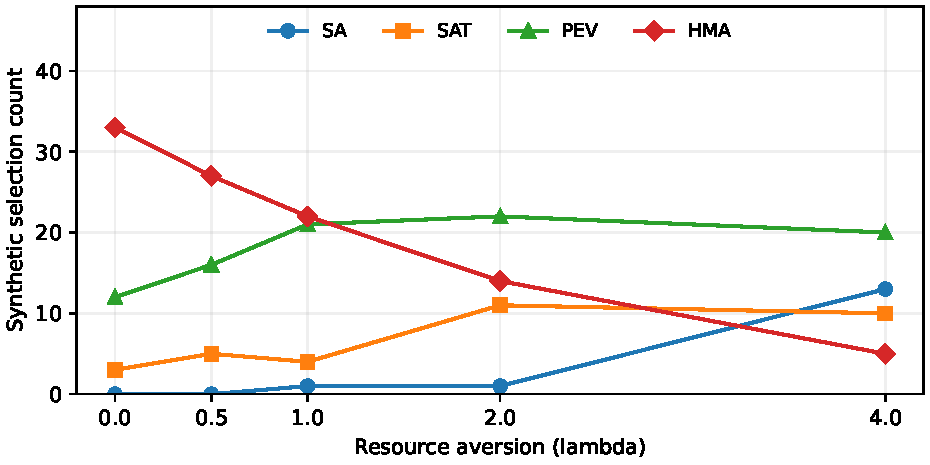
\includegraphics[width=.82\linewidth]{figures/sensitivity.pdf}
\caption{Sensitivity of simulated recommendation counts to resource aversion, with fixed scenarios and hypothetical coefficients.}\label{fig:sensitivity}
\end{figure}

As a controlled example, setting every feature to $0.5$ and $\lambda=1$ gives utilities $-0.020$, $0.100$, $0.275$, and $0.150$ for SA, SAT, PEV, and HMA. PEV therefore wins this specified example. Setting every feature to zero gives an exact four-way tie and triggers explicit resolution. Neither calculation predicts an outcome for a deployed agent system.

\section{Reproducibility and technical validation}
The repository\footnote{\url{https://github.com/GouthamSiripuram/agent-architecture-selection}} includes the coefficient dictionary, seeded generator, supplied scenarios, tests, and notebook. Run \texttt{python scripts/reproduce\_paper.py} from its root to regenerate the coefficients table, sensitivity table, plot, and row-level utilities. Validation documentation records software versions and data hashes. The supplied scenario file is compared with freshly generated records, rather than relying on a matching filename.

Code inspection confirms the v0.2 finite/range validation and independent generation procedure. Version 0.3.0 adds validation for the tie tolerance and regression tests for exact ties and the analytical example. Technical validation verifies the implementation on these cases; it does not establish predictive accuracy. The prior seven-role assessment was an AI-assisted internal technical review, not independent human peer review.

\section{Empirical calibration protocol}
A future study should implement all architecture classes under a shared base model, tool set, task definition, and budget accounting scheme. Record success, token and monetary costs, elapsed time, communication, repeated work, and verification errors across repeated trials. Preserve failed attempts. Predefine a measured utility or constrained optimization target, rather than declaring the model's own argmax to be ground truth.

Elicit or estimate task descriptors without access to held-out outcomes. Fit coefficients and choose regularization only on training task families; use a separate validation split for feature and hyperparameter choices, then evaluate once on held-out families. Compare with always-single-agent, always-PEV, cheapest-feasible, and simple task-feature baselines. Report utility regret relative to the best measured architecture within the tested set, with task-level uncertainty. Such an oracle is itself uncertain when run counts are small.

Ablations should remove one feature at a time, compare fixed versus fitted coefficients, and test interaction terms. Sensitivity should cover descriptor noise, correlated task properties, model families, and budget levels. Any claim that the chosen descriptors predict architecture advantage remains a hypothesis until this protocol or an equivalent empirical study is executed.

\section{Discussion and limitations}
The reference coefficients partly encode the result: more complex classes receive larger decomposition benefits and larger resource penalties by construction. Uniform synthetic sampling may overrepresent unrealistic feature combinations. Linear additivity excludes thresholds, bottlenecks, and feature interactions. Architecture-conditioned coordination costs are reduced to a shared input and a scalar coefficient. Feature subjectivity can dominate the small utility differences that determine a recommendation. The four classes omit many possible implementations and do not isolate agent count from model capacity, tools, or prompting.

This artifact is therefore suitable for inspecting assumptions and building tests, not for making unsupervised production decisions. Calibration on one task family would not by itself establish generalization. No confidence interval, statistical significance claim, or benchmark win is inferred from the 48 deterministic scenario rows.

\section{Responsible use and AI assistance}
Architecture choice should respect task-specific authorization and safety constraints independently of utility. A favorable score cannot justify broadening tool permissions or removing human oversight. Future experiments should minimize sensitive trace retention and disclose task and budget exclusions.

Generative-AI tools assisted with drafting, editing, code review, and internal technical validation. Goutham Siripuram is the sole human author and is responsible for the manuscript, software, references, and scientific claims. AI assistance and the internal review do not constitute independent peer review.

\section{Conclusion}
The proposed model makes a coordination-adjusted architecture preference executable and inspectable. Synthetic calculations expose the implications of the reference coefficients and resource-aversion parameter. Determining whether the descriptors or recommendations are useful for real systems requires independently measured outcomes, calibration, and held-out evaluation.
\begingroup\small\sloppy\bibliographystyle{plain}\bibliography{references}\endgroup
\end{document}
